%%
%% Copyright 2007-2020 Elsevier Ltd
%%
%% This file is part of the 'Elsarticle Bundle'.
%% ---------------------------------------------
%%
%% It may be distributed under the conditions of the LaTeX Project Public
%% License, either version 1.2 of this license or (at your option) any
%% later version.  The latest version of this license is in
%%    http://www.latex-project.org/lppl.txt
%% and version 1.2 or later is part of all distributions of LaTeX
%% version 1999/12/01 or later.
%%
%% The list of all files belonging to the 'Elsarticle Bundle' is
%% given in the file `manifest.txt'.
%%
%% Template article for Elsevier's document class `elsarticle'
%% with harvard style bibliographic references

%\documentclass[preprint,12pt,authoryear]{elsarticle}

%% Use the option review to obtain double line spacing
%% \documentclass[authoryear,preprint,review,12pt]{elsarticle}

%% Use the options 1p,twocolumn; 3p; 3p,twocolumn; 5p; or 5p,twocolumn
%% for a journal layout:
%% \documentclass[final,1p,times,authoryear]{elsarticle}
% \documentclass[final,1p,times,twocolumn,authoryear]{elsarticle}
%% \documentclass[final,3p,times,authoryear]{elsarticle}
\documentclass[final,3p,times,twocolumn,authoryear]{elsarticle}
%\documentclass[a4paper,12pt]{article}
%% \documentclass[final,5p,times,authoryear]{elsarticle}
%% \documentclass[final,5p,times,twocolumn,authoryear]{elsarticle}

%% For including figures, graphicx.sty has been loaded in
%% elsarticle.cls. If you prefer to use the old commands
%% please give \usepackage{epsfig}
%\input{glyphtounicode}
%\pdfgentounicode=1

%% The amssymb package provides various useful mathematical symbols
\usepackage{amssymb}
\usepackage{multirow}
%\usepackage[xcolor,qtwo]{rvdtx}
%\usepackage{multicol}
\usepackage{color}
\usepackage{xspace}
\usepackage{pdfwidgets}
\usepackage{enumerate}
\usepackage{longtable}
\usepackage{supertabular}
%% The amsthm package provides extended theorem environments
%% \usepackage{amsthm}

%% The lineno packages adds line numbers. Start line numbering with
%% \begin{linenumbers}, end it with \end{linenumbers}. Or switch it on
%% for the whole article with \linenumbers.
%% \usepackage{lineno}

\journal{Radiation Physics and Chemistry}

\begin{document}

\begin{frontmatter}

%% Title, authors and addresses

%% use the tnoteref command within \title for footnotes;
%% use the tnotetext command for theassociated footnote;
%% use the fnref command within \author or \affiliation for footnotes;
%% use the fntext command for theassociated footnote;
%% use the corref command within \author for corresponding author footnotes;
%% use the cortext command for theassociated footnote;
%% use the ead command for the email address,
%% and the form \ead[url] for the home page:
%% \title{Title\tnoteref{label1}}
%% \tnotetext[label1]{}
%% \author{Name\corref{cor1}\fnref{label2}}
%% \ead{email address}
%% \ead[url]{home page}
%% \fntext[label2]{}
%% \cortext[cor1]{}
%% \affiliation{organization={},
%%            addressline={},
%%            city={},
%%            postcode={},
%%            state={},
%%            country={}}
%% \fntext[label3]{}

\title{Microwave induced transformation of defect subsystem in SiC and GaAs}


%\author[label1]{Oleg Olikh\corref{cor1}}
%\ead{olegolikh@knu.ua}
%\affiliation[label1]{organization={Physics Faculty, Taras Shevchenko National University of Kyiv},%Department and Organization
%            addressline={64/13, Volodymyrska Street},
%            city={Kyiv},
%            postcode={01601},
%            country={Ukraine}}
%\author[label2]{Petro Lytvyn}
%\affiliation[label2]{organization={V. Lashkaryov Institute of Semiconductor Physic of NAS of Ukraine},%Department and Organization
%            addressline={41, pr. Nauki},
%            city={Kyiv},
%            postcode={03028},
%            country={Ukraine}}
%\cortext[cor1]{Corresponding author}

\begin{abstract}
Text of abstract Text of abstract Text of abstract Text of abstract
Text of abstract Text of abstract Text of abstract Text of abstract
Text of abstract Text of abstract Text of abstract Text of abstract
Text of abstract Text of abstract Text of abstract Text of abstract
Text of abstract Text of abstract Text of abstract Text of abstract
\end{abstract}

%%Graphical abstract
%\begin{graphicalabstract}
%%\includegraphics{grabs}
%\end{graphicalabstract}

%Research highlights
%\begin{highlights}
%\item Research highlight 1
%\item Research highlight 2
%\end{highlights}

\begin{keyword}
Microwave
\sep SiC
\sep GaAs
\sep Defect transformation
\end{keyword}

\end{frontmatter}

%% \linenumbers

%% main text
\section{Introduction}\label{sec1}



It is well known (\cite{KozlovsEn,RadiationEffectsBook})

(\cite{MW:Rev,ZOHM2000,BHUNIA1998,Bacherikov2003En,Pashkov1994En,
BoltovetsEn,Milenin1994En,BelyaevIntac,ASHKINADZE1996,ProcSPIE,Belyaev1998JTFEn,
Bacherikov2008En,Konakova2015En,Konakova2012FTPEn}.)


 \cite{MW:Rev,ZOHM2000}

\cite{MW:Rev}

\cite{MW:Rev,BHUNIA1998}

\cite{BoltovetsEn,Pashkov1994En,Milenin1994En,BelyaevIntac,ProcSPIE,Konakova2015En,Konakova2012FTPEn}

\cite{Bacherikov2003En}

\cite{Bacherikov2003En,Belyaev1998JTFEn,Konakova2015En}

\cite{Milenin1994En}

\cite{Belyaev1998JTFEn}

\cite{Bacherikov2008En}

\cite{BelyaevIntac,ProcSPIE,Belyaev1998JTFEn}


\section{Experimental details}\label{sec2}

\cite{BoltovetsEn,Milenin1994En,BelyaevIntac,ASHKINADZE1996,ProcSPIE}


\begin{figure}
\center
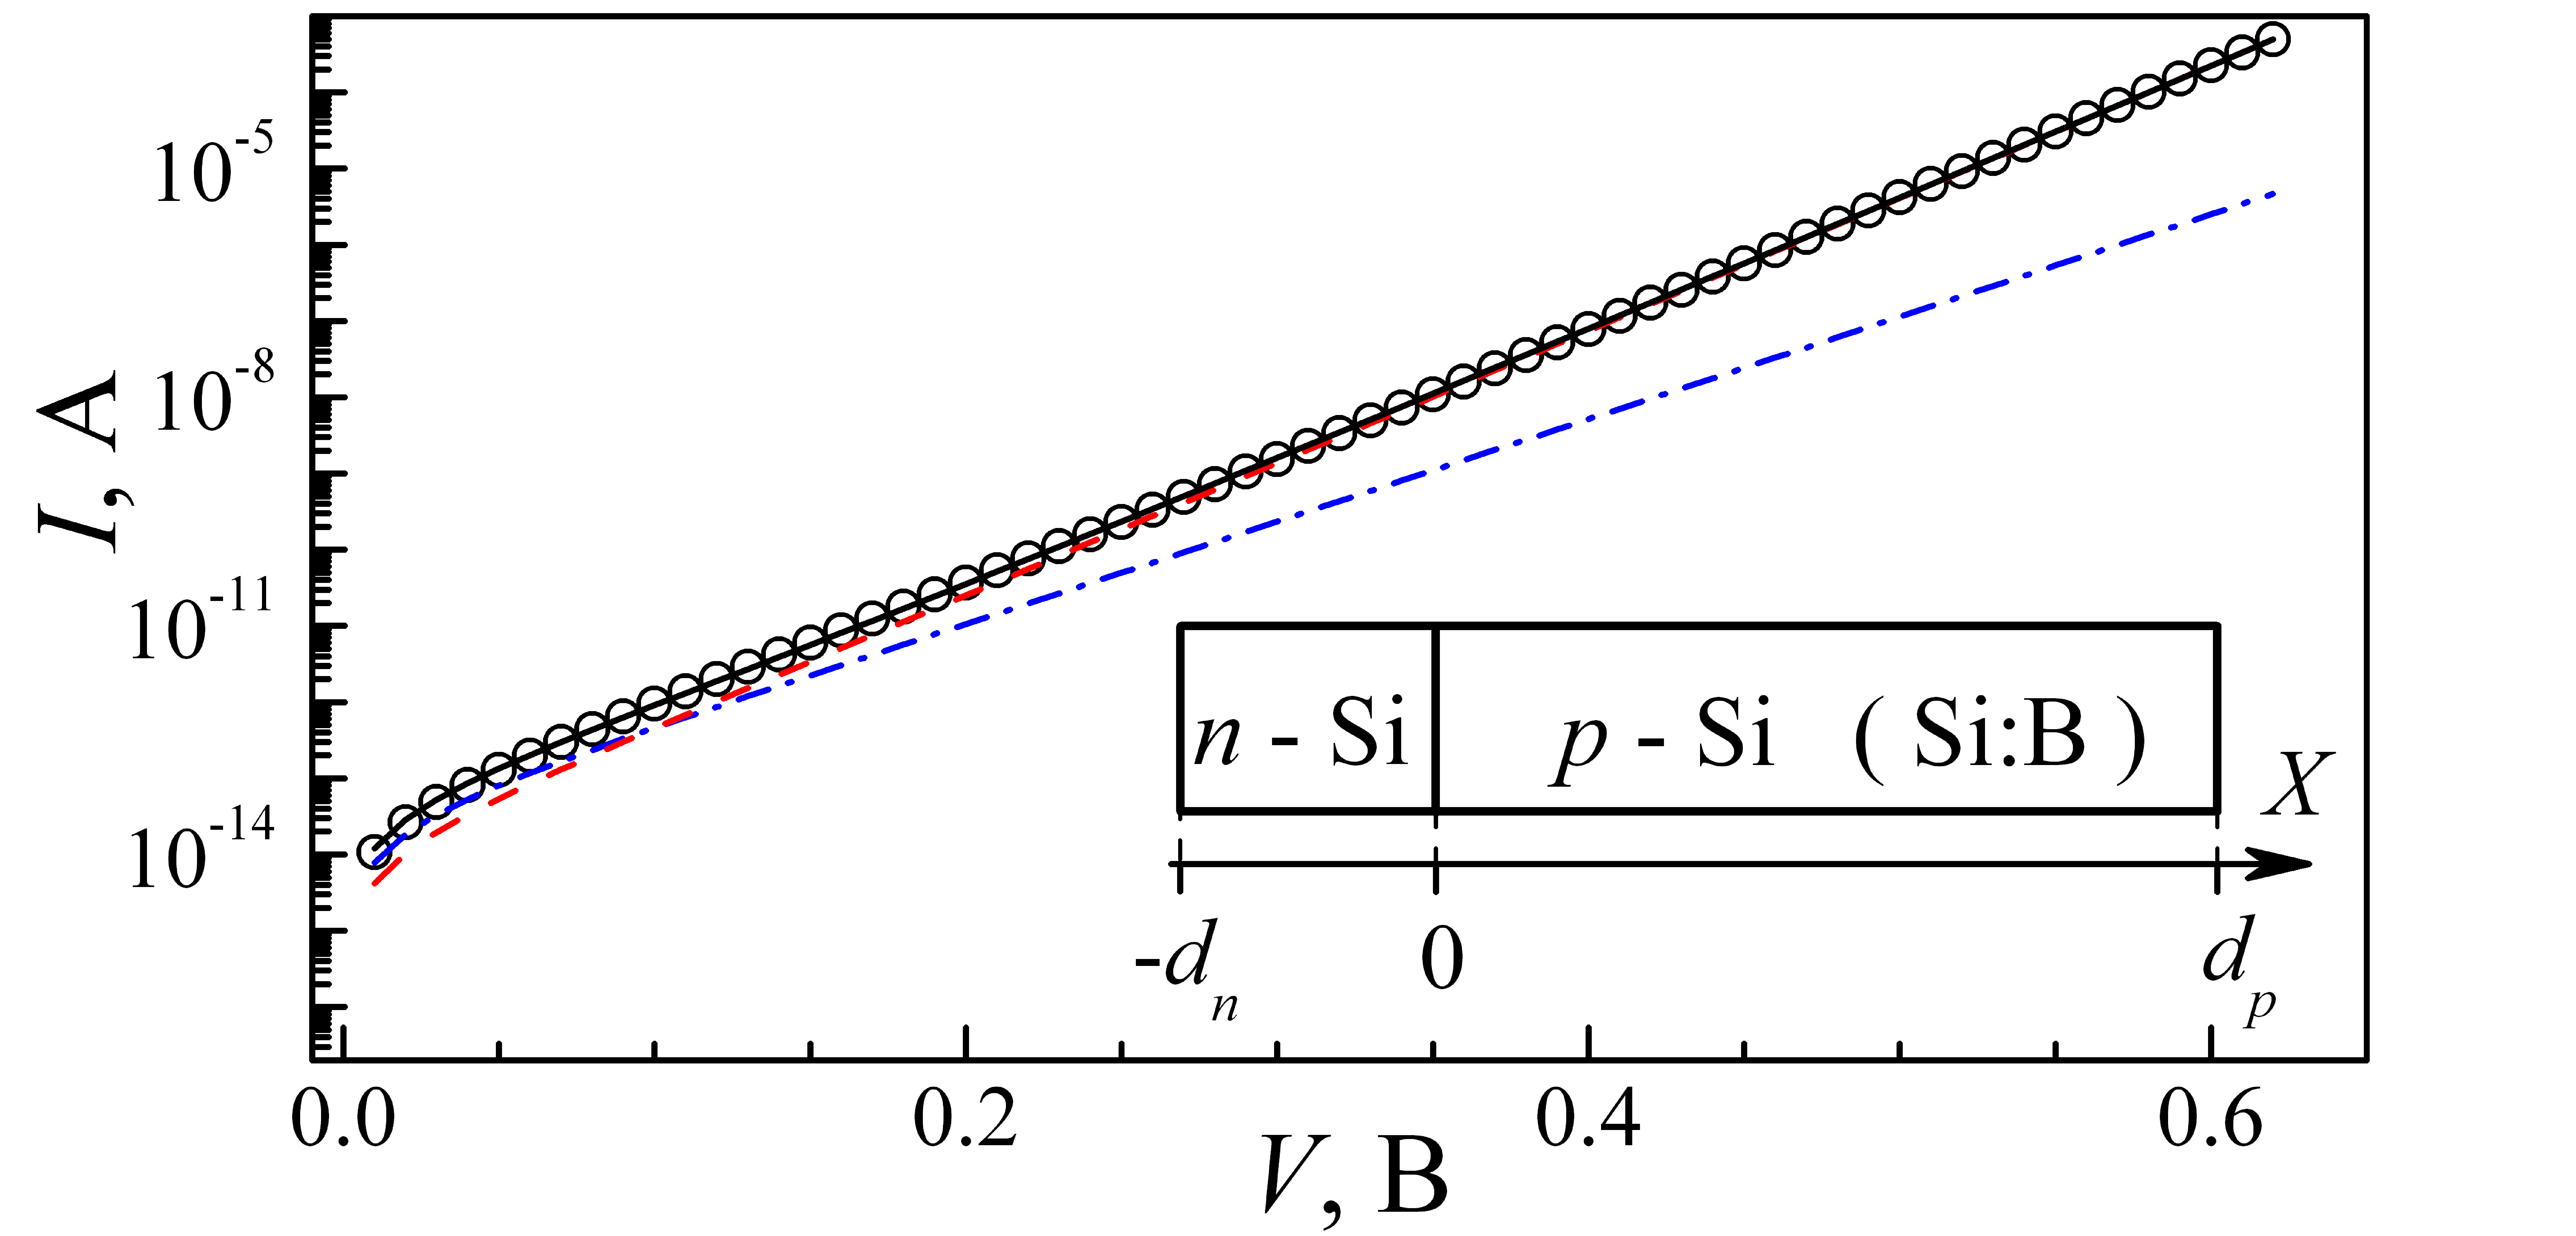
\includegraphics[width=0.5\textwidth]{Fig1}
\caption{\label{figSamp_TAV}
Structure of samples}%
\end{figure}


\cite{OstrovPAN,OlikhSSC,PANnewEn,OstrovskiiSST}

\begin{equation}\label{eqVtav}
  V_\mathtt{TAV}(t)=V_{\mathtt{TAV},0}\exp(-t/\tau).
\end{equation}


\begin{figure}
\center
\includegraphics[width=0.5\textwidth]{fig2}
\caption{\label{figTAV}
The scheme of TAV measurement.
The time dependencies of the radio impulse $V_\mathtt{RF}$ for the excitation of ultrasound in a piezoelectric plate and the resulting TAV signal $V_\mathtt{TAV}$ are schematically shown as well.
}%
\end{figure}


\cite{OstrovPAN,OstrovskiiSST}

\begin{equation}\label{eqPANtau}
  \tau=\frac{1}{\sigma_n\,\upsilon_{\mathrm{th},n}\,N_c}\exp\left(\frac{E_c-E_t}{kT}\right).
\end{equation}
where
$\upsilon_{\mathrm{th},n}$ is the electron thermal velocity
$N_C$ is the densities of states in the conduction band.


\cite{Godwod}

%\cite{ThoricBook}

\cite{Belyaev1998JTFEn}

\section{Results and discussion}\label{sec3}


\begin{figure*}
\center
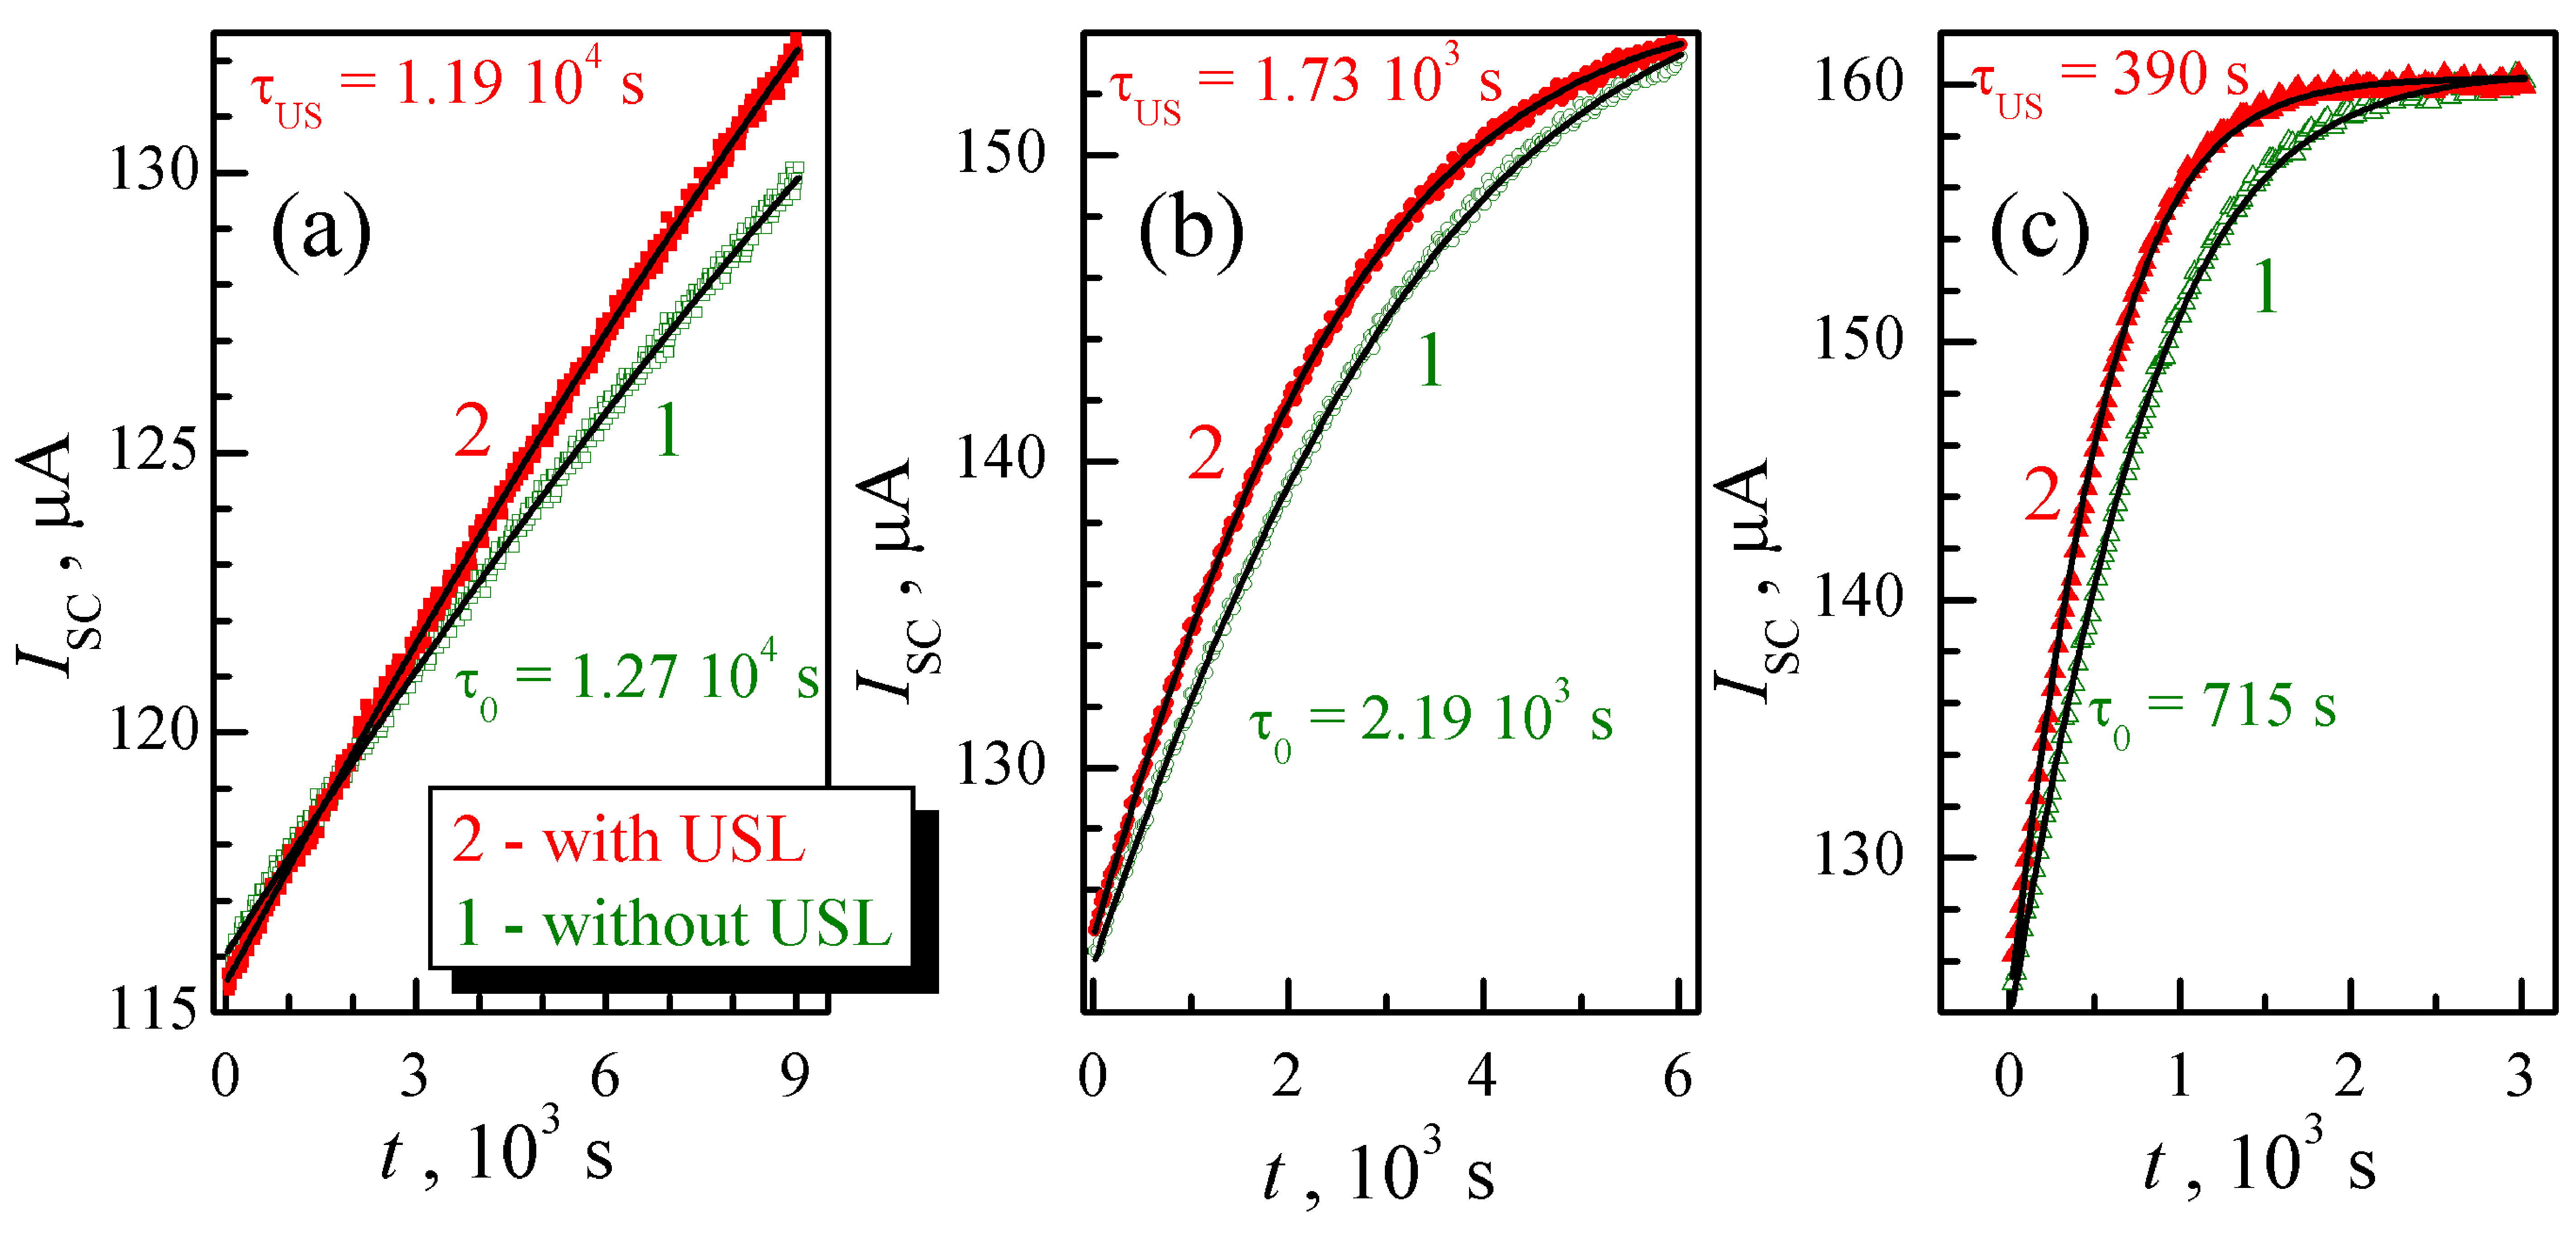
\includegraphics[width=0.7\textwidth]{Fig3}
\caption{\label{figTauTAV}
Dependences of TAV relaxation time on inverse temperature for samples SIC2 (a), SIC3 (b), GAS2 (c), GAE2 (d) and GAB1 (e) before and after MWT.
$t_\mathtt{MWT}$, c: 0 (curves 1), 20 (2), 40 (3), 60 (4)
}%
\end{figure*}


%\begin{table}
%  \caption{This is a test caption.}
%  \begin{tabular*}{\tblwidth}{@{} LLLL@{} }
%   \toprule
%    Col 1 & Col 2\\
%   \midrule
%    12345 & 12345\\
%    12345 & 12345\\
%    12345 & 12345\\
%    12345 & 12345\\
%    12345 & 12345\\
%    12345 & 12345\\
%   \bottomrule
%  \end{tabular*}
%\end{table}

\begin{table*}
\caption{\label{tabMW}The determined parameters of defects in the samples $n$--GaAs and $n$--6$H$--SiC samples
}
\center
%\renewcommand{\arraystretch}{0.95}
\begin{tabular}{ccccccc}
%\begin{tabular*}{\tblwidth}{@{} CCCCCCC@{}}
%\toprule
\hline
Sample& $t_\mathrm{MWT}$, s &Level &$(E_c-E_t)$, eV &$\sigma_n$, cm$^2$\textsuperscript{ a)}&$R_\mathrm{cur}$, m&$\xi_\mathrm{cur}$\\
%\midrule
\hline
SIC1& 0 &ESC1& $0.33\pm0.01$ &$(7\pm4)\cdot10^{-18}$&$\infty$&0\\ %\cline{2-7}
& 20 &ESC1& $0.33\pm0.01$ &$(5\pm3)\cdot10^{-19}$&170.2&$8.7\cdot10^{-7}$\\ %\cline{2-7}
& 40 &ESC2& $0.26\pm0.01$ &$(2\pm1)\cdot10^{-19}$&\multicolumn{2}{c}{\multirow{2}{*}{-}}\\ %\cline{2-5}
& 80 & \multicolumn{3}{c}{weak signal}&\multicolumn{2}{c}{}\\ %\hline
SIC2& 0 &ESC1& $0.33\pm0.01$ &$(7\pm4)\cdot10^{-18}$&$>2000$&$<1.2\cdot10^{-7}$\\ %\cline{2-7}
& 20 &ESC1& $0.33\pm0.01$ &$(5\pm3)\cdot10^{-19}$&171.9&$1.4\cdot10^{-6}$\\ %\hline
SIC3& 0 &ESC1& $0.34\pm0.02$ &$(3\pm2)\cdot10^{-18}$&3.8&$6.1\cdot10^{-5}$\\ %\cline{2-7}
& 20 &ESC2&$0.29\pm0.01$ &$(5\pm3)\cdot10^{-19}$&5.5&$4.2\cdot10^{-5}$\\ %\cline{2-7}
& 40 &ESC2& $0.26\pm0.01$ &$(10\pm7)\cdot10^{-20}$&\multicolumn{2}{c}{\multirow{2}{*}{-}}\\ %\cline{2-5}
& 80 &ESC2& $0.23\pm0.01$ &$(6\pm4)\cdot10^{-20}$&\multicolumn{2}{c}{}\\ %\hline
GAS1& 0 &EGA1& $0.32\pm0.02$ &$(3\pm2)\cdot10^{-17}$&-53.8&$-2.8\cdot10^{-6}$\\ %\cline{2-7}
& 20 &EGA1& $0.31\pm0.01$ &$(2\pm1)\cdot10^{-17}$&22.9&$6.5\cdot10^{-6}$\\ %\cline{2-7}
& 40 & \multicolumn{3}{c}{weak signal}&\multicolumn{2}{c}{-}\\ %\hline
GAS2& 0 &EGA1& $0.32\pm0.01$ &$(4\pm2)\cdot10^{-17}$&17.2&$8.7\cdot10^{-6}$\\ %\cline{2-7}
& 20 &EGA2& $0.28\pm0.01$ &$(5\pm2)\cdot10^{-18}$&14.7&$1.0\cdot10^{-5}$\\ %\cline{2-7}
& 40 & \multicolumn{3}{c}{weak signal}&\multicolumn{2}{c}{}\\ %\cline{1-5}
GAT& 0 &EGA3& $0.49\pm0.02$ &$(5\pm3)\cdot10^{-14}$&\multicolumn{2}{c}{}\\ %\cline{2-5}
& 20 &EGA4& $0.40\pm0.02$ &$(2\pm1)\cdot10^{-15}$&\multicolumn{2}{c}{}\\ %\cline{1-5}
GAE1& 0 &EGA5& $0.24\pm0.01$ &$(2\pm1)\cdot10^{-18}$&\multicolumn{2}{c}{}\\ %\cline{2-5}
& 60 &EGA2& $0.29\pm0.01$ &$(10\pm6)\cdot10^{-18}$&\multicolumn{2}{c}{}\\ %\cline{1-5}
GAE2& 0 &EGA5& $0.25\pm0.01$ &$(2\pm1)\cdot10^{-18}$&\multicolumn{2}{c}{}\\ %\cline{2-5}
& 60 &EGA2& $0.30\pm0.01$ &$(2\pm1)\cdot10^{-17}$&\multicolumn{2}{c}{}\\ %\cline{1-5}
GAE3& 0 &EGA6& $0.43\pm0.01$ &$(8\pm5)\cdot10^{-17}$&\multicolumn{2}{c}{-}\\ %\cline{2-5}
& 60 &EGA6& $0.46\pm0.02$ &$(7\pm4)\cdot10^{-16}$&\multicolumn{2}{c}{}\\ %\cline{1-5}
GAB1& 0 &EGA4& $0.39\pm0.01$ &$(10\pm7)\cdot10^{-18}$&\multicolumn{2}{c}{}\\ %\cline{2-5}
& 20 &EGA4& $0.39\pm0.01$ &$(4\pm2)\cdot10^{-17}$&\multicolumn{2}{c}{}\\ %\cline{2-5}
& 40 &EGA6& $0.43\pm0.02$ &$(10\pm6)\cdot10^{-17}$&\multicolumn{2}{c}{}\\ %\cline{1-5}
GAB2& 0 &EGA4& $0.40\pm0.01$ &$(10\pm6)\cdot10^{-17}$&\multicolumn{2}{c}{}\\ %\cline{2-5}
& 20 &EGA4& $0.41\pm0.01$ &$(10\pm6)\cdot10^{-17}$&\multicolumn{2}{c}{}\\ %\cline{2-5}
& 40 &EGA6& $0.45\pm0.02$ &$(4\pm2)\cdot10^{-16}$&\multicolumn{2}{c}{}\\  %\hline
\multicolumn{6}{l}{\textsuperscript{ a)} \emph{at $T=300$~K for SIC, GA, GAE and at $T=340$~K for GAB}}\\
\hline
%\bottomrule
\end{tabular}
\end{table*}

 \cite{Pavlovic2000}

\cite{Bulyarskii2000,Makram}

\cite{Stellmacher}

\cite{Bourgoin2001}

\cite{Bourgoin2001}

\cite{Bourgoin:GaAs}

\cite{Pavlovic2000}

\cite{Lebed1999En,Anikin1991:2En,Anikin1991:3En}

\cite{Kuznets1997En}

\cite{Lebed1999En}

\cite{Lebed1999En}

\cite{Anikin1991:2En,Anikin1991:3En}

\cite{Lebedev2000En}

\cite{Lebedev2001En}

\cite{Hemmingsson}

\cite{Lebedev2001En}

\pagebreak

%\begin{table*}
%\caption{\label{tabEGA1}Literature data for levels closed to the location of detected levels
%}
%\center
%\begin{tabular}{cccccc}
%\hline
%$(E_c-E_t)$, eV &$\sigma_n$, cm$^2$&configuration&method$\textsuperscript{ a)}$&epi--structure&Reference\\
%\hline
%\multicolumn{6}{c}{EGA1, ($E_c-E_t)=(0.31\div0.32)$~eV}\\
%0.33&-&complex with V$_\mathrm{As}$&DLTS&no&\cite{EL6:Richter}\\% \hline
%0.33&-&-&DLTS&no&\cite{Neild1991}\\ %\hline
%$0.31\div0.33$&-&V$_\mathrm{As}$&&no&\cite{EL6:Schultz}\\ %\hline
%0.33&$1\cdot10^{-17}$&-&TSC&no&\cite{Pavlovic2000}\\ %\hline
%0.323&$1\cdot10^{-14}$&-&DLTS&yes&\cite{Yousefi1995}\\ %\hline
%0.334&$2\cdot10^{-15}$&&DLTS&yes&\cite{Yousefi1995}\\ %\hline
%0.35&-&complex with V$_\mathrm{As}$&PA&no&\cite{EL6:Kuisma}\\ %\hline
%$0.315\div0.325$&$3\cdot10^{-17}$&-&TSC&no&\cite{Pavlovic:GaAs}\\ %\hline
%0.33&-&-&TSC&no&\cite{Tomozane:GaAs}\\ %\hline
%$0.30\div0.33$&-&-&DLTS&no&\cite{Lang:GaAs}\\ %\hline
%\multicolumn{6}{c}{EGA2, ($E_c-E_t)=(0.28\div0.30)$~eV}\\
%0.28&$5\cdot10^{-18}$&V$_\mathrm{As}$As$_i$&TSC&no&\cite{Pavlovic2000}\\ %\hline
%0.26&$3.5\cdot10^{-15}$&-&DLTS&yes&\cite{Yousefi1995}\\ %\hline
%0.277&$5\cdot10^{-17}$&-&TSC&no&\cite{Pavlovic:GaAs}\\ %\hline
%0.284&$1\cdot10^{-17}$&-&TSC&no&\cite{Pavlovic:GaAs}\\ %\hline
%0.28&-&intrinsic&TP&no&\cite{Abele:GaAs}\\ %\hline
%0.28&$8\cdot10^{-15}$&-&DLTS&yes&\cite{Mircea1975}\\ %\hline
%0.30&-&complex with Te&DLTS&no&\cite{KolFTP1994En}\\ %\hline
%0.30&$6\cdot10^{-15}$&V$_\mathrm{As}$As$_i$&DLTS&no&\cite{Pons}\\ %\hline
%\multicolumn{6}{c}{EGA3, ($E_c-E_t)=0.49$~eV}\\
%0.50&-&Sb$_\mathrm{Ga}$&DLTS&no&\cite{Samoilov1994En}\\ %\hline
%0.48&$4\cdot10^{-16}$&As$_\mathrm{Ga}^{++}$&TSC&no&\cite{Pavlovic2000}\\ %\hline
%0.485&$2\cdot10^{-16}$&-&TSC&no&\cite{Pavlovic:GaAs}\\ %\hline
%0.48&-&impurity&TP&no&\cite{Abele:GaAs}\\ %\hline
%0.51&$1\cdot10^{-12}$&-&DLTS&no&\cite{Martin1977}\\ %\hline
%0.48&$3\cdot10^{-13}$&-&DLTS&no&\cite{Lang:GaAs}\\ %\hline
%0.50&$1\cdot10^{-15}$&V$_\mathrm{As}$, V$_\mathrm{Ga}$Ga$_i$V$_\mathrm{As}$ &DLTS&no&\cite{Pons}\\
%\multicolumn{6}{c}{EGA4, ($E_c-E_t)=(0.39\div0.41)$~eV}\\
%0.42&-&-&DLTS&no&\cite{Neild1991}\\ %\hline
%0.41&-&V$_\mathrm{Ga}$V$_\mathrm{As}$&DLTS&no&\cite{Samoilov1994En}\\ %\hline
%$0.39$&-&V$_\mathrm{Ga}$Ga$_\mathrm{As}$&TSC&no&\cite{FANG1990}\\ %\hline
%$0.41$&$2\cdot10^{-13}$&-&DLTS&yes&\cite{Bourgoin:GaAs}\\ %\hline
%0.40&-&-&SCRC&yes&\cite{ASHBY:GaAs}\\ %\hline
%0.37&$2\cdot10^{-14}$&-&DLTS&yes&\cite{Fang:EL6}\\ %\hline
%0.40&-&V$_\mathrm{Ga}$Ga$_\mathrm{As}$&DLTS&no&\cite{VaitkusEn}\\ %\hline
%0.387&$2\cdot10^{-14}$&-&DLTS&yes&\cite{Yousefi1995}\\ %\hline
%\multicolumn{6}{c}{EGA5, ($E_c-E_t)=(0.24\div0.25)$~eV}\\
%0.23&-&-&DLTS&no&\cite{Neild1991}\\ %\hline
%0.23&$2\cdot10^{-17}$&-&TSC&no&\cite{Pavlovic2000}\\ %\hline
%$0.22\div0.25$&$8\cdot10^{-19}$&-&TSC&no&\cite{Lin:GaAs}\\ %\hline
%$0.26$&-&complex with V$_\mathrm{Ga}$&TSC&no&\cite{FANG1990}\\ %\hline
%0.24&-&-&TSC&no&\cite{Tomozane:GaAs}\\ %\hline
%0.23&-&intrinsic&TP&no&\cite{Abele:GaAs}\\ %\hline
%0.23&-&V$_\mathrm{Ga}$V$_\mathrm{As}$&DLTS&no&\cite{Morrow:EL17}\\ %\hline
%0.23&$1\cdot10^{-14}$&V$_\mathrm{Ga}$V$_\mathrm{As}$&DLTS&no&\cite{Bourgoin:GaAs}\\ %\hline
%0.23&$7\cdot10^{-15}$&-&DLTS&yes&\cite{Mircea1975}\\ %\hline
%0.22&$2\cdot10^{-15}$&-&DLTS&no&\cite{Fang:EL6}\\ %\hline
%0.258&$4\cdot10^{-16}$&-&DLTS&yes&\cite{Yousefi1995}\\ %\hline
%\multicolumn{6}{c}{EGA6, ($E_c-E_t)=(0.43\div0.46)$~eV}\\
%0.44&$1\cdot10^{-14}$&V$_\mathrm{As}$As$_i$, V$_\mathrm{As}$&TSC&no&\cite{Pavlovic2000}\\ %\hline
%0.44&$9\cdot10^{-15}$&-&TSC&no&\cite{Pavlovic:GaAs}\\ %\hline
%\multirow{2}{*}{0.43}&\multirow{2}{*}{$7\cdot10^{-16}$}&\multirow{2}{*}{intrinsic}&\multirow{2}{*}{DLTS}&\multirow{2}{*}{yes}&\cite{Lefevre1977}\\
%&&&&&\cite{Bourgoin:GaAs}\\
%%0.43&$7\cdot10^{-16}$&intrinsic&DLTS&yes&\cite{Lefevre1977} \cite{Bourgoin:GaAs}\\ %\hline
%0.44&$2\cdot10^{-15}$&complex with V$_\mathrm{As}$&DLTS&yes&\cite{KolFTP1989En}\\ %\hline
%\multicolumn{6}{l}{$\textsuperscript{ a)}$ \emph{DLTS --- deep level transient spectroscopy}}\\
%%\multicolumn{6}{l}{ \emph{TSC --- метод термостимульованих струмів}}\\
%%\multicolumn{6}{l}{ \emph{PA --- позитрон--анігіляційна спектроскопія}}
%%\multicolumn{6}{l}{\emph{TP --- релаксація фотопровідності}}
%%\multicolumn{6}{l}{\emph{SCRC --- температурна залежність струму ОПЗ}}\\
%\hline
%\end{tabular}
%\end{table*}


\begin{table*}
\caption{\label{tabEGA1}Literature data for levels closed to the location of detected levels
}
\center
\begin{minipage}{1.85\textwidth}
\begin{tabular}{cccccc}
\hline
$(E_c-E_t)$, eV &$\sigma_n$, cm$^2$&configuration&method$\textsuperscript{ a)}$&epi--structure&Reference\\
\hline
\multicolumn{6}{c}{EGA1, ($E_c-E_t)=(0.31\div0.32)$~eV}\\
0.33&-&complex with V$_\mathrm{As}$&DLTS&no&\cite{EL6:Richter}\\% \hline
0.33&-&-&DLTS&no&\cite{Neild1991}\\ %\hline
$0.31\div0.33$&-&V$_\mathrm{As}$&&no&\cite{EL6:Schultz}\\ %\hline
0.33&$1\cdot10^{-17}$&-&TSC&no&\cite{Pavlovic2000}\\ %\hline
0.323&$1\cdot10^{-14}$&-&DLTS&yes&\cite{Yousefi1995}\\ %\hline
0.334&$2\cdot10^{-15}$&&DLTS&yes&\cite{Yousefi1995}\\ %\hline
0.35&-&complex with V$_\mathrm{As}$&PA&no&\cite{EL6:Kuisma}\\ %\hline
$0.315\div0.325$&$3\cdot10^{-17}$&-&TSC&no&\cite{Pavlovic:GaAs}\\ %\hline
0.33&-&-&TSC&no&\cite{Tomozane:GaAs}\\ %\hline
$0.30\div0.33$&-&-&DLTS&no&\cite{Lang:GaAs}\\ %\hline
\multicolumn{6}{c}{EGA2, ($E_c-E_t)=(0.28\div0.30)$~eV}\\
0.28&$5\cdot10^{-18}$&V$_\mathrm{As}$As$_i$&TSC&no&\cite{Pavlovic2000}\\ %\hline
0.26&$3.5\cdot10^{-15}$&-&DLTS&yes&\cite{Yousefi1995}\\ %\hline
0.277&$5\cdot10^{-17}$&-&TSC&no&\cite{Pavlovic:GaAs}\\ %\hline
0.284&$1\cdot10^{-17}$&-&TSC&no&\cite{Pavlovic:GaAs}\\ %\hline
0.28&-&intrinsic&TP&no&\cite{Abele:GaAs}\\ %\hline
0.28&$8\cdot10^{-15}$&-&DLTS&yes&\cite{Mircea1975}\\ %\hline
0.30&-&complex with Te&DLTS&no&\cite{KolFTP1994En}\\ %\hline
0.30&$6\cdot10^{-15}$&V$_\mathrm{As}$As$_i$&DLTS&no&\cite{Pons}\\ %\hline
\multicolumn{6}{c}{EGA3, ($E_c-E_t)=0.49$~eV}\\
0.50&-&Sb$_\mathrm{Ga}$&DLTS&no&\cite{Samoilov1994En}\\ %\hline
0.48&$4\cdot10^{-16}$&As$_\mathrm{Ga}^{++}$&TSC&no&\cite{Pavlovic2000}\\ %\hline
0.485&$2\cdot10^{-16}$&-&TSC&no&\cite{Pavlovic:GaAs}\\ %\hline
0.48&-&impurity&TP&no&\cite{Abele:GaAs}\\ %\hline
0.51&$1\cdot10^{-12}$&-&DLTS&no&\cite{Martin1977}\\ %\hline
0.48&$3\cdot10^{-13}$&-&DLTS&no&\cite{Lang:GaAs}\\ %\hline
0.50&$1\cdot10^{-15}$&V$_\mathrm{As}$, V$_\mathrm{Ga}$Ga$_i$V$_\mathrm{As}$ &DLTS&no&\cite{Pons}\\
\multicolumn{6}{c}{EGA4, ($E_c-E_t)=(0.39\div0.41)$~eV}\\
0.42&-&-&DLTS&no&\cite{Neild1991}\\ %\hline
0.41&-&V$_\mathrm{Ga}$V$_\mathrm{As}$&DLTS&no&\cite{Samoilov1994En}\\ %\hline
$0.39$&-&V$_\mathrm{Ga}$Ga$_\mathrm{As}$&TSC&no&\cite{FANG1990}\\ %\hline
$0.41$&$2\cdot10^{-13}$&-&DLTS&yes&\cite{Bourgoin:GaAs}\\ %\hline
0.40&-&-&SCRC&yes&\cite{ASHBY:GaAs}\\ %\hline
0.37&$2\cdot10^{-14}$&-&DLTS&yes&\cite{Fang:EL6}\\ %\hline
0.40&-&V$_\mathrm{Ga}$Ga$_\mathrm{As}$&DLTS&no&\cite{VaitkusEn}\\ %\hline
0.387&$2\cdot10^{-14}$&-&DLTS&yes&\cite{Yousefi1995}\\ %\hline
\multicolumn{6}{c}{EGA5, ($E_c-E_t)=(0.24\div0.25)$~eV}\\
0.23&-&-&DLTS&no&\cite{Neild1991}\\ %\hline
0.23&$2\cdot10^{-17}$&-&TSC&no&\cite{Pavlovic2000}\\ %\hline
$0.22\div0.25$&$8\cdot10^{-19}$&-&TSC&no&\cite{Lin:GaAs}\\ %\hline
$0.26$&-&complex with V$_\mathrm{Ga}$&TSC&no&\cite{FANG1990}\\ %\hline
0.24&-&-&TSC&no&\cite{Tomozane:GaAs}\\ %\hline
0.23&-&intrinsic&TP&no&\cite{Abele:GaAs}\\ %\hline
0.23&-&V$_\mathrm{Ga}$V$_\mathrm{As}$&DLTS&no&\cite{Morrow:EL17}\\ %\hline
0.23&$1\cdot10^{-14}$&V$_\mathrm{Ga}$V$_\mathrm{As}$&DLTS&no&\cite{Bourgoin:GaAs}\\ %\hline
0.23&$7\cdot10^{-15}$&-&DLTS&yes&\cite{Mircea1975}\\ %\hline
0.22&$2\cdot10^{-15}$&-&DLTS&no&\cite{Fang:EL6}\\ %\hline
0.258&$4\cdot10^{-16}$&-&DLTS&yes&\cite{Yousefi1995}\\ %\hline
\multicolumn{6}{c}{EGA6, ($E_c-E_t)=(0.43\div0.46)$~eV}\\
0.44&$1\cdot10^{-14}$&V$_\mathrm{As}$As$_i$, V$_\mathrm{As}$&TSC&no&\cite{Pavlovic2000}\\ %\hline
0.44&$9\cdot10^{-15}$&-&TSC&no&\cite{Pavlovic:GaAs}\\ %\hline
\multirow{2}{*}{0.43}&\multirow{2}{*}{$7\cdot10^{-16}$}&\multirow{2}{*}{intrinsic}&\multirow{2}{*}{DLTS}&\multirow{2}{*}{yes}&\cite{Lefevre1977}\\
&&&&&\cite{Bourgoin:GaAs}\\
%0.43&$7\cdot10^{-16}$&intrinsic&DLTS&yes&\cite{Lefevre1977} \cite{Bourgoin:GaAs}\\ %\hline
0.44&$2\cdot10^{-15}$&complex with V$_\mathrm{As}$&DLTS&yes&\cite{KolFTP1989En}\\ %\hline
\multicolumn{6}{l}{$\textsuperscript{ a)}$ \emph{DLTS --- deep level transient spectroscopy}}\\
%\multicolumn{6}{l}{ \emph{TSC --- метод термостимульованих струмів}}\\
%\multicolumn{6}{l}{ \emph{PA --- позитрон--анігіляційна спектроскопія}}
%\multicolumn{6}{l}{\emph{TP --- релаксація фотопровідності}}
%\multicolumn{6}{l}{\emph{SCRC --- температурна залежність струму ОПЗ}}\\
\hline
\end{tabular}
\end{minipage}
\end{table*}

\cite{KolFTP1994En}

\cite{Samoilov1994En}

\cite{VaitkusEn}

\cite{KolFTP1989En}

\cite{Konakova2007JTFEn}

\cite{BoltovetsEn,Konakova2012FTPEn}

\cite{Bacherikov2003En,Pashkov1994En,BoltovetsEn,Milenin1994En,BelyaevIntac}

\cite{ZOHM2000}

\cite{FANG1990}

\cite{OstrovskiiSST,OlikhSSC,OstrovPAN}

\cite{BoltovetsEn,Konakova2012FTPEn}

\cite{Yousefi1995,Mircea1975,Bourgoin:GaAs,ASHBY:GaAs,Fang:EL6,Lefevre1977,KolFTP1989En}


%% The Appendices part is started with the command \appendix;
%% appendix sections are then done as normal sections
%% \appendix

%% \section{}
%% \label{}

%% If you have bibdatabase file and want bibtex to generate the
%% bibitems, please use
%\bibliographystyle{elsarticle-num}
%\bibliographystyle{cas-model2-names}
%\bibliographystyle{elsarticle-num-names}

\section*{References}
\bibliographystyle{elsarticle-harv}
\bibliography{olikh}


\end{document}

\endinput
%%
%% End of file `elsarticle-template-harv.tex'.
